\documentclass[letterpaper]{article}
\usepackage{amsmath}
\usepackage{tikz}
\usepackage{epigraph}
\usepackage{lipsum}
\usepackage{hyperref}
\usepackage{tocloft}
\usepackage{graphicx}
\usepackage{float}

\usepackage{setspace, amsmath}

\usepackage[centering,includeheadfoot,margin=2cm]{geometry}
\usepackage{xcolor}
\usepackage{calc,blindtext}

\renewcommand\epigraphflush{flushright}
\renewcommand\epigraphsize{\normalsize}
\setlength\epigraphwidth{0.6\textwidth}

\definecolor{titlepagecolor}{cmyk}{1,.60,0,.40}

\DeclareFixedFont{\titlefont}{T1}{ppl}{b}{it}{1.0in}

\makeatletter
\def\printauthor{%
    {\large \@author}}
\makeatother
\author{%
    Nico Taljaard \\
    10153285 \vspace{20pt} \\
    Gerhard Smit \\
    12282945 \vspace{20pt} \\
    Martin Schoeman \\
    10651994 \\
}

% The following code is borrowed from: http://tex.stackexchange.com/a/86310/10898

\newcommand\titlepagedecoration{%
	\begin{tikzpicture}[remember picture,overlay,shorten >= -10pt]
	
		\coordinate (aux1) at ([yshift=-15pt]current page.north east);
		\coordinate (aux2) at ([yshift=-410pt]current page.north east);
		\coordinate (aux3) at ([xshift=-4.5cm]current page.north east);
		\coordinate (aux4) at ([yshift=-150pt]current page.north east);
		
		\begin{scope}[titlepagecolor!40,line width=12pt,rounded corners=12pt]
			\draw
			  (aux1) -- coordinate (a)
			  ++(225:5) --
			  ++(-45:5.1) coordinate (b);
			\draw[shorten <= -10pt]
			  (aux3) --
			  (a) --
			  (aux1);
			\draw[opacity=0.6,titlepagecolor,shorten <= -10pt]
			  (b) --
			  ++(225:2.2) --
			  ++(-45:2.2);
		\end{scope}
			\draw[titlepagecolor,line width=8pt,rounded corners=8pt,shorten <= -10pt]
			  (aux4) --
			  ++(225:0.8) --
			  ++(-45:0.8);
		\begin{scope}[titlepagecolor!70,line width=6pt,rounded corners=8pt]
			\draw[shorten <= -10pt]
			  (aux2) --
			  ++(225:3) coordinate[pos=0.45] (c) --
			  ++(-45:3.1);
			\draw
			  (aux2) --
			  (c) --
			  ++(135:2.5) --
			  ++(45:2.5) --
			  ++(-45:2.5) coordinate[pos=0.3] (d);   
			\draw 
			  (d) -- +(45:1);
		\end{scope}
	\end{tikzpicture}
}

\begin{document}

\begin{titlepage}

\noindent
\titlefont Laminin \par
\epigraph{ XGame - Derivco \\ Corspe Slasher \\ Functional requirements and application design.}%
{\textit{ 01/08/2014 }\\ \textsc{ }}
\null\vfill
\vspace*{4cm}
\noindent
\hfill
\begin{minipage}{0.35\linewidth}
    \begin{flushright}
        \printauthor
    \end{flushright}
\end{minipage}
%
\begin{minipage}{0.02\linewidth}
    \rule{1pt}{125pt}
\end{minipage}
\titlepagedecoration
\end{titlepage}

% % % % % % % % % % % % % % %
% 							%
%	Remainder of document	%
% 							%
% % % % % % % % % % % % % % % 

	\newpage
		{\LARGE \bf Change Log}\\[2em]
		
		\begin{tabbing}
			\hspace*{2.5cm}\=\hspace*{2.5cm}\=\hspace*{8cm}\=\hspace*{3cm} \kill
			28/07/2014	\> Version 1.0	\> Document Created 							\> Nico Taljaard \\
			29/07/2014	\> Version 1.0	\> Added game class diagram						\> Nico Taljaard \\
			29/07/2014	\> Version 1.0	\> Added game use case diagram					\> Nico Taljaard \\
			30/07/2014	\> Version 1.1	\> Change document structure					\> Nico Taljaard \\
		\end{tabbing}
		
	\newpage
		\renewcommand\contentsname{TABLE OF CONTENTS}
		\newcommand\contentsnameLC{\colorbox{blue}{\makebox[\textwidth-2\fboxsep][l]{\bfseries\color{white} Table of Contents}}}
		
		\renewcommand{\cftdot}{}
		\hypersetup{linktocpage}
		\tableofcontents
		
		\begin{flushleft}
			\LARGE\href{https://github.com/njTaljaard/Laminin_CorpseSlasher/}{Git repository: Laminin - Corpse Slasher}
		\end{flushleft}
		
	\newpage
		
		\section*{\colorbox{blue}{\makebox[\textwidth-2\fboxsep][l]{\bfseries\color{white} Functional Requirements }}} \addcontentsline{toc}{section}{Functional Requirements}
		\vspace{0.1in}
		
			\subsection*{Introduction:}
			\addcontentsline{toc}{subsection}{Introduction}
			\vspace{0.1in}
			
			
			
			\vspace{0.2in}
			\subsection*{Required Functionality:}
			\addcontentsline{toc}{subsection}{Required Functionality}
			\vspace{0.1in}
			
				\subsubsection*{Game Diagrams:}
				\addcontentsline{toc}{subsubsection}{Game Diagrams}
				\vspace{0.2in}
				
					\begin{figure}[H]
					\centering
					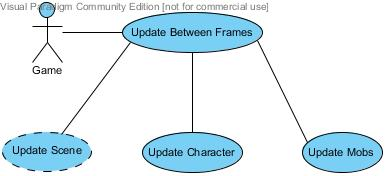
\includegraphics[width=140mm]{UML_Diagram/Use_Case/Game_Process.jpg}
					\caption{Update process between frames}
					\end{figure}
					
					\begin{figure}[H]
					\centering
					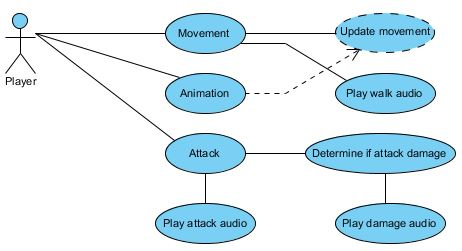
\includegraphics[width=140mm]{UML_Diagram/Use_Case/Player_Actions.jpg}
					\caption{Actions available to player}
					\end{figure}
					
					\begin{figure}[H]
					\centering
					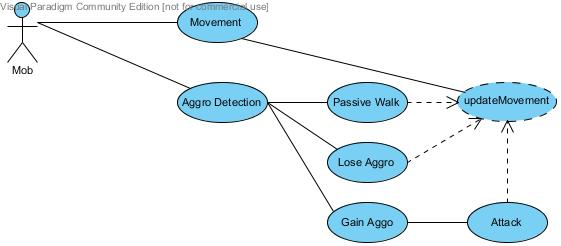
\includegraphics[width=140mm]{UML_Diagram/Use_Case/Mob_Actions.jpg}
					\caption{Actions available to mobs}
					\end{figure}
					
					\begin{figure}[H]
					\centering
					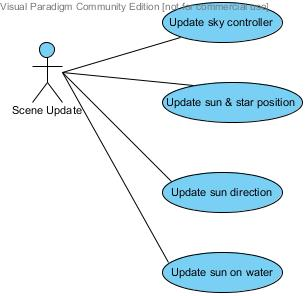
\includegraphics[width=140mm, height=100mm]{UML_Diagram/Use_Case/Update_Scene.jpg}
					\caption{Update of scene elements}
					\end{figure}
					
				\vspace{0.2in}
				\subsubsection*{User-interface Diagrams:}
				\addcontentsline{toc}{subsubsection}{User-interface Diagrams}
				\vspace{0.2in}
				
				
				
				\vspace{0.2in}
				\subsubsection*{Server Diagrams:}
				\addcontentsline{toc}{subsubsection}{Server Diagrams}
				\vspace{0.2in}
				
				
				
			\vspace{0.2in}
			\subsection*{Use Case prioritization:}
			\addcontentsline{toc}{subsection}{Use Case prioritization / services contracts}
			\vspace{0.1in}
					
				\subsubsection*{Critical:}
				\addcontentsline{toc}{subsubsection}{Critical}
				\vspace{0.1in}
					
					\begin{itemize}
						\item Update process between frames.
						\item Update of scene elements.
					\end{itemize}	
					
				\vspace{0.2in}
				\subsubsection*{Important:}
				\addcontentsline{toc}{subsubsection}{Important}
				\vspace{0.2in}
				
					\begin{itemize}
						\item Actions available to player
						\item Actions available to mobs
					\end{itemize}
				
				\vspace{0.2in}
				\subsubsection*{Nice-To-Have:}
				\addcontentsline{toc}{subsubsection}{Nice-To-Have}
				\vspace{0.2in}
					
			\vspace{0.2in}
			\subsection*{Use Case services contracts:}
			\addcontentsline{toc}{subsection}{Use Case prioritization / services contracts}
			\vspace{0.1in}
				
				\subsubsection*{Game Diagrams:}
				\addcontentsline{toc}{subsubsection}{Game Diagrams}
				\vspace{0.1in}
					
					\hspace{5mm}Update process between frames
					\begin{itemize}
						\item Pre-Conditions: \\
							Game is still running within the main game loop. \\
							Update time is provided from game engine defining the uptime of game. \\
							Player character is not null and initialized to be update. \\
							Mob characters is not null and initialized to be update.
						\item Post-Conditions: \\
							Game scene has updated as defined in update scene elements. \\
							Character action updated as defined in actions of player. \\
							Mobs actions updated as defined in actions of mob.
						\item Request and Results Data Structures \\
							
					\end{itemize}
					
					\vspace{0.1in}
					Actions available to player
					\begin{itemize}
						\item Pre-Condition: \\
							Character handler is not null and initialized. \\
							Character repositioning direction available from the directional keys pressed. \\
							Player animations channel is retrieved from model and can be updated. \\
							Player attack registered for process.
						\item Post-Condition: \\
							Character position has been updated according to direction of movement and movement speed. \\
							Player animation has been set successfully to animations channel with define loop state and play speed. \\
							Player attack action has occurred and processed between player and attacked mob.
						\item Request and Results Data Structures \\
							
					\end{itemize}
					
					\vspace{0.1in}
					Actions available to mobs
					\begin{itemize}
						\item Pre-Condition: \\
							Character handler is not null and initialized. \\
							Character repositioning direction is given from players position. \\
							Mob aggro detection is not null and attach to physics space. \\
							Mob aggro obtained flagged. \\
							Mob aggro loss flagged. \\
							Mob animation channel is retrieved from model and can be updated. \\
							Mob attack registered for process.
						\item Post-Condition: \\
							Character position updated to the direction of player and a distance of the movement speed. \\
							Mob aggro process and state updated for motion and animation loop. \\
							Mob animation has been set successfully to animations channel with define loop state and play speed. \\
							Mob attack action has occurred and processed between mob and player.
						\item Request and Results Data Structures \\
						
					\end{itemize}
					
					\vspace{0.1in}
					Update of scene elements
					\begin{itemize}
						\item Pre-Condition: \\
							Sky control not null and initialized. \\
							Update value provided from game engine of frame time.
						\item Post-Condition: \\
							Sun \& Stars updated by sky control. \\
							Sun direction updated retrieved from sky control and assigned to the light. \\
							Sun on the water updated from the new set light direction. \\
							Time of day updated through sky control.
						\item Request and Results Data Structures \\
						
					\end{itemize}
					
				\vspace{0.2in}
				\subsubsection*{User-interface Diagrams:}
				\addcontentsline{toc}{subsubsection}{User-interface Diagrams}
				\vspace{0.2in}
				
				
				
				\vspace{0.2in}
				\subsubsection*{Server Diagrams:}
				\addcontentsline{toc}{subsubsection}{Server Diagrams}
				\vspace{0.2in}
					
			\vspace{0.2in}
			\subsection*{Process specifications:}
			\addcontentsline{toc}{subsection}{Process specifications}
			\vspace{0.1in}
			
			
			
			\vspace{0.2in}
			\subsection*{Domain Objects:}
			\addcontentsline{toc}{subsection}{Domain Objects}
			\vspace{0.1in}
			
				\vspace{0.2in}
				\subsubsection*{Class Diagrams:}
				\addcontentsline{toc}{subsubsection}{Class Diagrams}
				\vspace{0.1in}
				
					\begin{figure}[H]
					\centering
					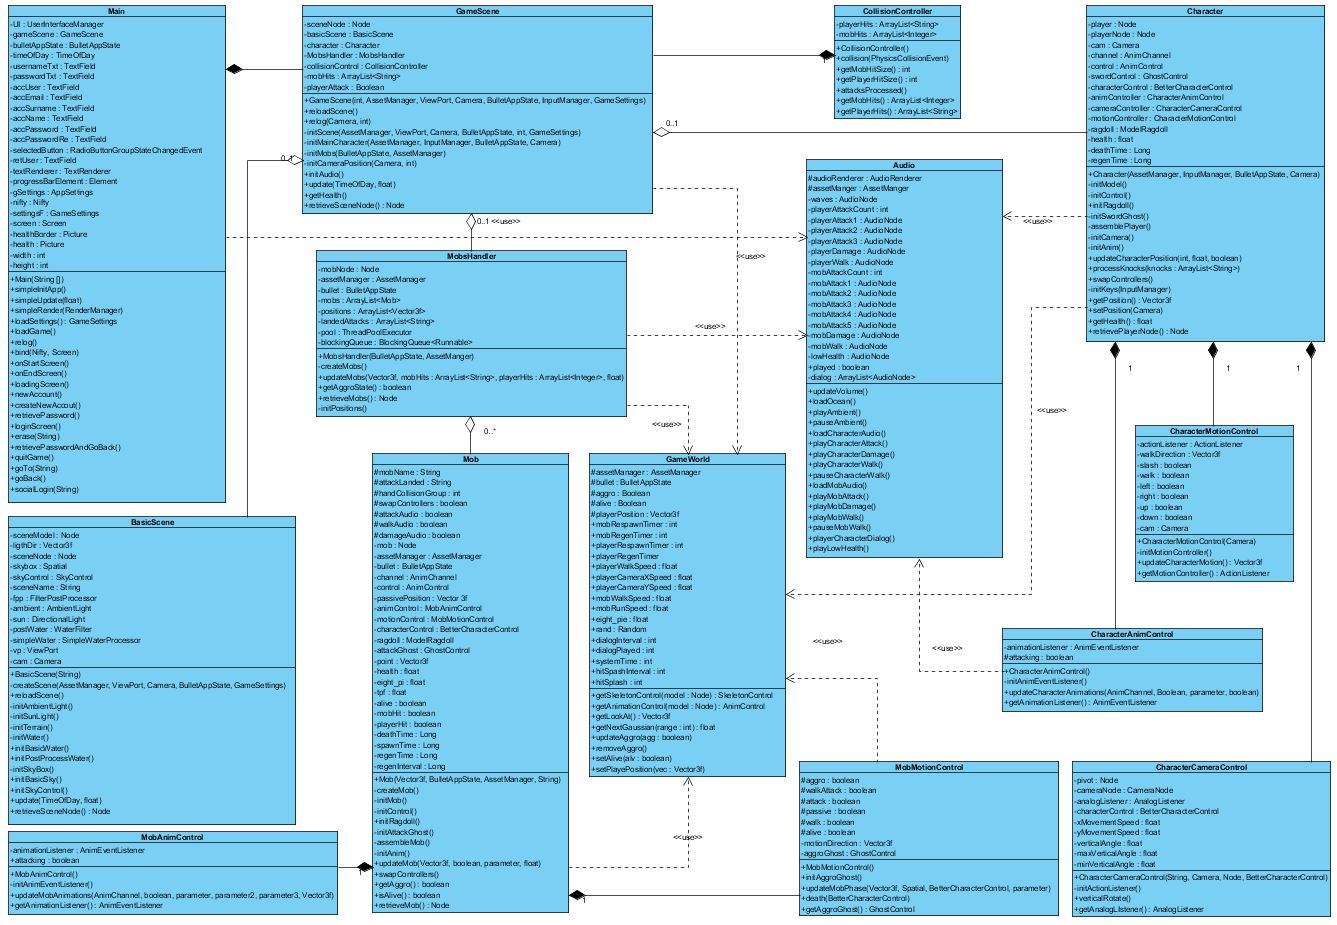
\includegraphics[width=180mm]{UML_Diagram/Class/Game_Classes.jpg}
					\caption{Game level class diagram}
					\label{overflow}
					\end{figure}
					
				\vspace{0.2in}
				\subsubsection*{State Diagrams:}
				\addcontentsline{toc}{subsubsection}{State Diagrams}
				\vspace{0.1in}
					
					
					
				\vspace{0.2in}
				\subsubsection*{Activity Diagrams:}
				\addcontentsline{toc}{subsubsection}{Activity Diagrams}
				\vspace{0.1in}
					
					
					
				\vspace{0.2in}
				\subsubsection*{ERD Diagrams:}
				\addcontentsline{toc}{subsubsection}{ERD Diagrams}
				\vspace{0.1in}
					
					
		\vspace{0.2in}
		
		\section*{\colorbox{blue}{\makebox[\textwidth-2\fboxsep][l]{\bfseries\color{white} Application Design }}} \addcontentsline{toc}{section}{Application Design}
		\vspace{0.1in}
		
		
		
		\vspace{0.2in}
		
		\section*{\colorbox{blue}{\makebox[\textwidth-2\fboxsep][l]{\bfseries\color{white} Code Documentation }}} \addcontentsline{toc}{section}{Code Documentation}
		\vspace{0.1in}
		
			\subsection*{Game documentation:}
			\addcontentsline{toc}{subsection}{Game documentation}
			\vspace{0.1in}
			
			\vspace{0.2in}
			\subsection*{User-interface documentation:}
			\addcontentsline{toc}{subsection}{User-interface documentation}
			\vspace{0.1in}
			
			\vspace{0.2in}
			\subsection*{Server documentation:}
			\addcontentsline{toc}{subsection}{Server documentation}
			\vspace{0.1in}
		
		\vspace{0.2in}
		
\end{document}